\documentclass{letask}
\usepackage{hyperref}
\usepackage{parskip}
\usepackage{graphicx}

\begin{document}
\begin{titlepage}
\center % Center everything on the page
 
%----------------------------------------------------------------------------------------
%	HEADING SECTIONS
%----------------------------------------------------------------------------------------

\textsc{\LARGE Московский\\[-0.2cm]Физико-Технический Институт\\[0.1cm]\large (государственный университет)}\\[1.5cm] % Name of your university/college
\textsc{\Large Кафедра общей физики}\\[0.1cm] % Major heading such as course name
\textsc{\large Вопрос по выбору, 2 семестр}\\[0.5cm] % Minor heading such as course title

%----------------------------------------------------------------------------------------
%	TITLE SECTION
%----------------------------------------------------------------------------------------

\HRule
\\[0.4cm]
{ \huge \bfseries Оценка времени рассеяния\\[0.2cm]
	атмосферы планет}
\\[0.6cm] % Title of your document
\HRule
\\[1.5cm]


 
%----------------------------------------------------------------------------------------
%	AUTHOR SECTION
%----------------------------------------------------------------------------------------

\begin{minipage}{0.4\textwidth}
	\begin{flushleft} \large
		\textsf{Студент}
		
		Павел \textsc{Северилов} \\[-0.15cm]
		671 группа
	\end{flushleft}
\end{minipage}
~
\begin{minipage}{0.4\textwidth}
	\begin{flushright} \large
		\textsf{Преподаватель}
		
		Владимир Александрович \\[-0.15cm]
		\textsc{Овчинкин} % Supervisor's Name
	\end{flushright}
\end{minipage}

\begin{bottompar}
	\begin{center}
		
\includegraphics[width = 80 mm]{logo.jpg}
	\end{center}
	{\large \today}

\end{bottompar}
\vfill % Fill the rest of the page with whitespace

\end{titlepage}


\textbf{Ввведение:} 

\parindent=0.5cm Применим закон распределения Больцмана к уединенной планете, окруженной газовой атмосферой, которую будем считать изотермической. Кроме того, будем предполагать, что все молекулы одинаковы, и что масса атмосферы пренебрежимо мала по сравнению с массой планеты. Тогда потенциальная энергия молекулы в поле тяготения планеты будет равна $GMm/r$. Для концентрации молекул $n$ на расстоянии $r$ от центра планеты закон Больцмана дает:
		\begin{gather}
			n=n_0\exp \frac{GMm}{kTr},
		\end{gather}
где $M$ -- масса планеты, а $G$ -- гравитационная постоянная. Если бы формула (1) была применима на всех расстояниях от планеты, то на бесконечности получилось бы конечное значение для концентрации $n$, а именно $n = n_0$. Но это невозможно, так как общее количество молекул в атмосфере планеты конечно, а объем пространства, окружающего ее, бесконечно велик. Равновесие возможно только при $n_0 = 0$, т е. при полном отсутствии атмосферы. 

\parindent=0.5cm Невозможность равновесного состояния планетной атмосферы связана с тем, что существуют молекулы, которые не могут удерживаться полем тяготения планеты, то есть такие молекулы, скорости которых превышают вторую космическую (скорость убегания молекулы). Такие молекулы всегда появляются в результате столкновений. Поэтому к планетной атмосфере в целом неприменима формула Больцмана, т.к. ее вывод предполагал, что газ находится в состоянии термодинамического равновесия. Пусть в некоторый момент скорости молекул в атмосфере распределены по закону Максвелла. Если бы с этого момента молекулы перестали сталкиваться между собой, то все молекулы, скорости которых превышают вторую космическую (убегающие молекулы), навсегда покинули бы планету. Остались бы только молекулы со скоростями, распределеными по закону Максвелла. Тогда для такой системы будет термодинамическое равновесие, и оно будет обязательно больцмановским. Т.к. для планеты достаточно большой массы доля молекул со скоростями, превышающими вторую космическую, ничтожна, то распределение частиц мы можем представить в данном виде: подавляющая доля молекул распределена в пространстве по закону Больцмана. На больцмановсксое распределение накладывается поток убегающих молекул. Вблизи планеты относительная концентрация убегающих молекул в таком потоке ничтожна. По мере удаления от планеты эта относительная концентрация непрерывно растет. На бесконечности все молекулы являются убегающими. Поток убегающих молекул непрерывно пополняется в результате межмолекулярных столкновений. Это приводит к тому, что планета в конце концов должна потерять атмосферу. Время $\tau$, в течение которого масса атмосферы планеты убывает в $e$ раз, называется временем рассеяния атмосферы.

\newpage
	\begin{center}
		\textbf{\Large{Оценка $\tau$}}
	\end{center}
	
\textbf{Часть 1:}

\parindent=0.5cmОценка времени рассеяния идеализированной изотермической атмосферы может дать результат, отличающийся на порядок и даже больше от действительного времени рассеяния. Однако такая оценка все же даст представление о порядке величины этого времени.

\parindent=0.5cm Опишем вокруг планеты сферу $\sigma$, концентрическую с поверхностью планеты. Радиус $r_{\sigma}$ этой сферы возьмем настолько большим, чтобы столкновениями между молекулами вне сферы $\sigma$ можно было полностью пренебречь, но этого нельзя делать в пространстве, ограниченном сферой $\sigma$. Введем две скорости убегания: на поверхности планеты и на сфере $\sigma$. Обозначим их соответственно через $v_0$ и $v_{\sigma}$. Если $r_0$ -- радиус планеты, $g_0$ и $g_{\sigma} = g_0 r^2_0/r^2_{\sigma}$ — ускорения свободного падения на поверхности планеты и на сфере $\sigma$, то 
		\begin{gather}
			v_0 = \sqrt{2g_0r_0}; \\
			v_{\sigma} = \sqrt{2g_\sigma r_\sigma} = r_0 \sqrt{2g_0/r_\sigma}
		\end{gather}
Величины $v_0$ и $v_\sigma$ связаны между собой уравнением энергии
	\begin{gather}
	\frac{mv^2_0}{2} = \frac{mv^2_\sigma}{2} + \varepsilon_p,
	\end{gather}
где $\varepsilon_p$ -- разность потенциальных энергий на сфере $\sigma$ и на поверхности планеты. Введем скорость $x = v/v_m$ -- безразмерная скорость, где $v_m = \sqrt \frac{2kT}{m}$ -- наиболее вероятная скорость. В частности, безразмерные скорости убегания на поверхности планеты и на сфере $\sigma$ равны $x_0 = v_0/v_m$ и $x_\sigma = v_\sigma/v_m$. Ввиду (2) и (3) они связаны соотношением 
	\begin{gather}
	x^2_\sigma = \frac{r_0}{r_\sigma}x^2_0.
	\end{gather}
Соотношение (4), записанное в безразмерных величинах, будет 
	\begin{gather}
	\frac{\varepsilon_p}{kT} = x^2_0 - x^2_\sigma.
	\end{gather}
С учетом соотношения (6) из закона распределения Больцмана получим 
	\begin{gather}
	n_\sigma e^{-x^2_\sigma} = n_0 e^{-x^2_0}
	\end{gather}
где $n_\sigma$ — концентрация молекул на сфере $\sigma$. Если пользоваться безразмерными скоростями, то максвелловское распределение $dn = 4\pi v^2 (\frac{m}{2 \pi kT})^{3/2} \exp(-\frac{mv^2}{2kT})$ примет вид
	\begin{gather}
	dn = n\frac{4}{\sqrt{\pi}}x^2e^{-x^2}dx.
	\end{gather}
Концентрация убегающих молекул на сфере $\sigma$ равна 
	\begin{gather}
	\Delta n = \frac{4n_\sigma}{\sqrt{\pi}}J,
	\end{gather}
где $J$ означает интеграл 
	\begin{gather}
	J = \int \limits_{x_\sigma}^{\infty} x^2e^{-x^2}\,dx.
	\end{gather}
Средняя безразмерная скорость таких молекул будет
	$$c \equiv \langle x \rangle_{x>x_\sigma} = \frac{1}{J} \int \limits_{x_\sigma}^{\infty} x^3e^{-x^2}\,dx.$$
Интегрируя это выражение по частям, получаем
	\begin{gather}
	c = \frac{1}{2J}(x^2_\sigma + 1)e^{-x^2_\sigma}
	\end{gather}
	
\parindent=0.5cm  Найдем средний поток убегающих частиц $Z$, исходящий наружу из сферы $\sigma$. Поскольку распределение скоростей молекул изотропно, можно воспользоваться формулой $z = \frac{n \langle v \rangle}{4}$. Средняя скорость рассматриваемых частиц, выраженная в обычных единицах, равна $cv_m$, а потому получаем $Z = (1/4)Scv_m\Delta n$, где  $ S = 4\pi r^2_\sigma$ -- поверхность сферы $\sigma$. Подставив сюда выражения (9) и (11) и воспользовавшись формулами (5) и (7), получим 
	\begin{gather}
	Z = 2\sqrt{\pi} \left(\frac{r_0}{r_\sigma}x^2_0 + 1\right) n_0r^2_\sigma v_m e^{-x^2_0}.
	\end{gather}
Это выражение и дает число молекул, теряемых атмосферой в единицу времени. Его можно представить в виде 
	\begin{gather}
	Z = -dN/dt,
	\end{gather}
где $N$ -- полное число молекул в атмосфере. Концентрацию $n_0$ можно выразить через $N$. Подавляющая масса атмосферы приходится на тонкий слой, примыкающий к поверхности планеты. В пределах этого слоя можно пренебречь кривизной поверхности планеты, а также изменением ускорения свободного падания с высотой, т е. положить $g = g_0$. Тогда распределение Больцмана переходит в барометрическую формулу, и мы получаем
	$$N = 4 \pi r^2_0 n_0 \int \limits_0^{\infty} exp\left(-\frac{mg_0z}{kT}\right)\,dz = 4 \pi r^2_0 n_0 \frac{kT}{mg_0}$$
Отсюда и найдется концентрация $n_0$. Подставляя ее в выражение (12) и воспользовавшись уравнением (13), придадим последнему вид 
	\begin{gather}
	dN/dt = -N/\tau,
	\end{gather}
где введено обозначение 
	\begin{gather}
	\tau = \frac{2\sqrt{\pi}r^2_0kT}{mg_0r^2_\sigma v_m \left(\frac{r_0}{r_\sigma}x^2_0 + 1\right)}e^{x^2_0}.
	\end{gather}
Интегрирование уравнения (14) дает $N = N_0e^{-t/\tau}.$ Из этой формулы видно, что постоянная $\tau$ есть введенное выше время рассеяния атмосферы.


\newpage

\textbf{Часть 2:}

Формула (15) еще не решает задачу, так как она содержит радиус $r_\sigma$, который мы еще не определили. В предельном случае, когда планетная атмосфера бесконечно разреженная, в ней полностью отсутствуют столкновения между молекулами, а распределение молекул в пространстве и по скоростям устанавливается в результате столкновений с поверхностью планеты. В рассматриваемом случае следует положить  $r_\sigma = r_0$. Используя, кроме того, соотношения $v_m^2 = 2kТ/m$ и $x_0v_m = v_0 = \sqrt{2r_0g_0}$, получим время рассеяния бесконечно разреженной атмосферы
	\begin{gather}
	\tau = \sqrt{\frac{2\pi r_0}{g_0}}\frac{e^{x^2_0}}{x_0(x_0^2+1)}
	\end{gather}
Также справедливо соотношение
	\begin{gather}
	\frac{\tau_0}{\tau_\sigma} = \frac{r_\sigma}{r_0},
	\end{gather}
где $\tau_0$ и $\tau_\sigma$ означают времена рассеяния, вычисленные по формуле для бесконечно разреженной атмосферы и по формуле (15) соответственно. Видно, что формула для бесконечно разреженной атмосферы (17) завышает время рассеяния всего в несколько раз. Поэтому дальнейшие численные расчеты будут произведены с помощью формулы (16), т.к. она дает вполне приемлимую оценку.

\parindent=0.5cm Однако формула (16) очень чувствительна к температуре атмосферы $T$, влияние которой сказывается преимущественно через экспoненциалыный множитель $e^{x_0^2}$ . А так как на разных высотах температура атмосферы разная и постоянно меняется, то невозможно с достаточной точностью определить значение $T$, которое следует подставлять в формулу. Поэтому воспользуемся формулой (16) для решения обратной задачи — по заданному времени $\tau$ найдем $x_0^2$, а затем и температуру планетной атмосферы, при которой она рассеивается в окружающее пространство за время $\tau$. Проведем расчет для $\tau = 10^{10}$ лет и $\tau = 10^8$ лет. Подставляя эти значения в формулу (16) и логарифмируя, получаем значения $x_0^2$. Температуру $T$ можем найти из соотношения $x_0^2 = \frac{2R_0g_0}{v_m^2} = \frac{R_0g_0}{kT}$:
	\begin{gather}
	T = \frac{R_0g_0m}{kx_0^2}
	\end{gather}
	
$$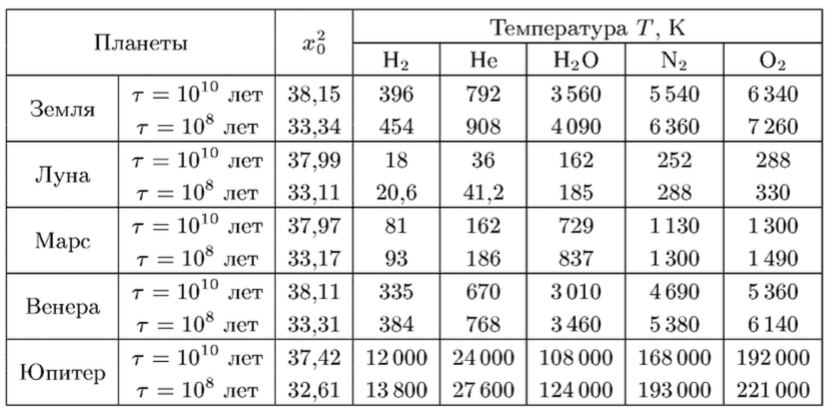
\includegraphics[scale=0.99]{11}$$

\newpage
\textbf{Итог:}

Из таблицы видно, что время $\tau$ очень чувствительно к изменениям температуры $Т$. При изменении $Т$ на $12-15\%$ $\tau$ меняется на два порядка. Отсюда следует, что рассеяние атмосферы должно сильно возрастать из-за нерегулярных местных колебаний температуры. Из таблицы видно, что поле тяготения Земли надежно удерживает в течение геологических эпох все газы земной атмосферы, за исключением водорода и гелия. Формула (18) объясняет, почему Луна практически лишена атмосферы, а мощное гравитационное поле Юпитера не позволяет в течение геологических эпох рассеяться сколько-нибудь заметно даже наиболее легкому газу -- водороду. Понятно также, почему Луна лишена атмосферы, а на Титане -- шестом спутнике Сатурна -- обнаружена атмосфера из метана, аммиака и других газов, хотя скорости убегания на обоих спутниках почти одинаковы (2,4 км/с на Луне и 2,6 км/с на Титане). Дело в том, что температура поверхности Титана (примерно 70-120 К) много ниже температуры лунной поверхности. При такой низкой температуре только наиболее легкие газы -- водород и гелий --
обладают тепловыми скоростями, достаточными для быстрого улетучивания их в окружающее пространство. Марс, имея меньшую, чем Земля, силу притяжения, из-за диссипации атмосферы потерял большую часть своей атмосферы. Из планет Солнечной системы наименее благоприятны условия для удержания атмосферы на Меркурии. Скорость убегания с поверхности планеты составляет всего 3,8 км/с. Неблагоприятны также крайне высокая температура на поверхности планеты и давление электромагнитного и корпускулярного излучения Солнца, которое способно заметно выдуватью молекулы газов из атмосферы Меркурия. Поэтому Меркурий могут покидать даже молекулы тяжелых газов.

\bigskip
\bigskip
\bigskip
\bigskip
\bigskip

\paragraph{Литература.} 
\begin{enumerate}
	\item Сивухин Д. В. Общий курс физики: Учеб. пособие: Для вузов. В 5 т. Т. II. Термодинамика и молекулярная физика. - 5-е изд., испр. - М.: ФИЗМАТЛИТ, 2005.
	\item \href{https://ru.wikipedia.org/wiki/Диссипация_атмосфер_планет}{https://ru.wikipedia.org/wiki/Диссипация$\textunderscore$атмосфер$\textunderscore$планет}
\end{enumerate}

\end{document}
